\documentclass[12pt]{standalone}

\usepackage{tikz}

\begin{document}
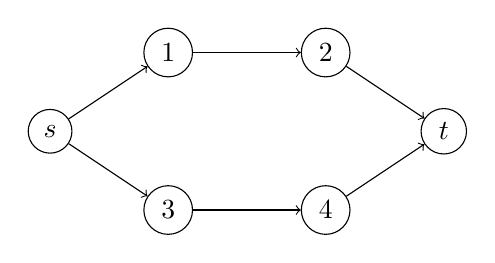
\begin{tikzpicture}

\begin{scope}[every node/.style={circle,draw}]
    \node (S) at (0,0) {$s$};
    \node (N1) at (1.5,1) {$1$};
    \node (N2) at (3.5,1) {$2$};
    \node (N3) at (1.5,-1) {$3$};
    \node (N4) at (3.5,-1) {$4$};
    \node (T) at (5,0) {$t$};
\end{scope}

\draw[->] (S) -- (N1);
\draw[->] (N1) -- (N2);
\draw[->] (N2) -- (T);
\draw[->] (S) -- (N3);
\draw[->] (N3) -- (N4);
\draw[->] (N4) -- (T);

\end{tikzpicture}
\end{document}
